%-------------------------------------------------------------------------
% Introduction (Brief Description of Topic + Fits in Field)
%-------------------------------------------------------------------------


\section{Introduction}

Artificial intelligence (AI) is a core tenant of video games, traditionally utilised as adversaries or opponents to human players. Likewise, game playing has long been a staple of AI research. However, academic research has traditionally focused mostly on board and card games and advances in game AI and academic AI have largely remained distinct.

The first video game opponents were simple discrete algorithms, such as the computer paddle in \emph{Pong}. In the late 1970s video game AIs became more advanced, utilising search algorithms and reacting to user input. In \emph{Pacman}, the ghost displayed distinct personalities and worked together against the human player \cite{pacmanghosts}. In the mid 1990s, approaches became more `agent' based. Finite State Machines (FSMs) emerged as a dominant game AI technique, as seen in games like \emph{Half-Life} \cite{halflife}. Later, in the 2000s, Behaviour Trees gained preeminence, as seen in games such as \emph{F.E.A.R.} \cite{fear} and \emph{Halo 2} \cite{halo}. These later advances borrowed little from contemporary development in academic AI and remained localised to the gaming industry.

In the last ten years, with increases in processing power and the complexity of games, many academic techniques have been harnessed by developers. For example, Monte Carlo Tree Search techniques developed in Go AI research have been used in \emph{Total War: Rome II} \cite{rome}. In 2008's \emph{Left 4 Dead}, Player Modelling was used to alter play experience for different users \cite[p.~10]{playermod}. Furthermore, AI and related techniques are no longer only being used as adversaries. There has been a rise in intelligent Procedural Content Generation in games in recent years, in both a game-world sense (for example \emph{MineCraft} and \emph{Terraria}) and also a story sense (for example \emph{Skyrim's} Radiant Quest System) \cite{skyrim}.

However, machine learning has yet to find a meaningful contribution to the world of video gaming, despite being a staple of academic research into AI, especially in robotics and board games. High complexity, small datasets and time constraints greatly hinder the effective implementation of learning techniques in the industry.

Conversely, commercial games have recently enjoyed more consideration in academic research. Games such as \emph{Ms. Pac Man}, \emph{Starcraft}, \emph{Unreal Tournament}, \emph{Super Mario Bros.} and open-source counterparts \emph{TORCS} \cite{torcs} and \emph{Cellz} \cite{cellz} have been at the centre of recent competitions and papers \cite{panorama} \cite{marioaicomp}. These competitions tend to focus on agent-based game-playing AI, with many entrants adopting an evolutionary learning approach. This research could have applications as AI `competitors' to human players, which is especially relevant to the racing, FPS and RTS genres.

This project will combine the notions of game-playing agents, evolutionary learning and traditional video game AI. By considering similar existing work, an evolutionary agent will be produced that learns to effectively play a 2D platforming game.


%-----------------------------------------------------------------------
% Definitions
%-----------------------------------------------------------------------
\subsection{Concept Definitions}
\label{subsec:concepts}

At this point it is useful to introduce some high level descriptions/definitions of some key concepts that will be used in this report.

\subsubsection{Intelligent Agents (IAs)}

\begin{figure}[t]
	\centering
	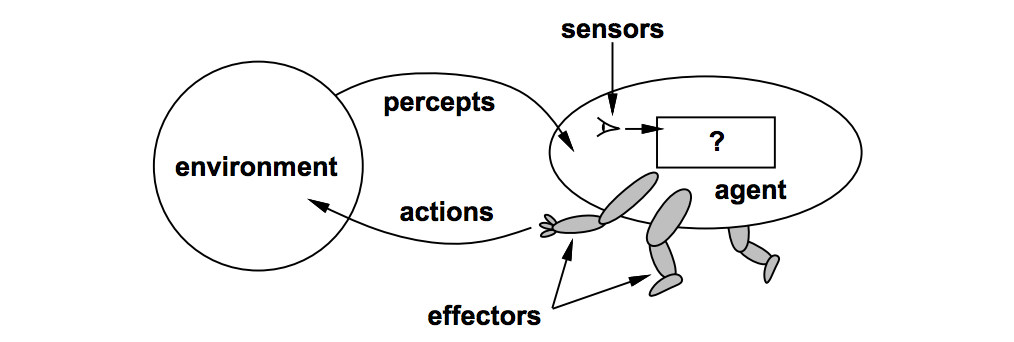
\includegraphics[scale=0.6]{intelligentagent.png}
	\caption{Illustration of an intelligent agent, taking from \cite[p.~32]{modernai1}}
	\label{fig:ia}
\end{figure}

An intelligent agent is an entity that uses \textbf{sensors} to perceive its \textbf{environment} and acts based on that perception through \textbf{actuators} or \textbf{effectors}. In software, this is often realised as an autonomous program or module that takes its perception of the \textbf{environment} as input an returns \textbf{actions} as output. Figure \ref{fig:ia} shows the basic structure of an intelligent agent. \cite[p.~34]{modernai3}


\subsubsection{Rule-based systems}

A rule-based system decides \textbf{actions} from \textbf{inputs} as prescribed by a \textbf{ruleset} or \textbf{rule base}. A \textbf{semantic reasoner} is used to manage to the relationship between input and the ruleset. This follows a \textbf{match-resolve-act} cycle, which first finds all rules matching an input, chooses one based on a conflict strategy and then uses the rule to act on the input, usually in the form of an output. \cite[pp.~28-29]{rbsys}

\subsubsection{Biologically Inspired Learning} 

Several computational learning approaches have derived their inspiration from learning in animals and humans. Two such approaches are relevant to this project: Reinforcement learning, strategy modelled on simplistic interpretation of how animal learn behaviour from their environment \cite[s.~1.2]{suttonrl}; and evolutionary computation, algorithms that apply Darwinian principles of evolution \cite{ev-comp}.


\subsubsection*{Reinforcement Learning}

A reinforcement learning agent focuses on a learning problem, with its goal to maximise \textbf{reward}. Given a current \textbf{state} the agent chooses an \textbf{action} available to it, which is determined by a \textbf{policy}. This action maps the current \textbf{state} to a new \textbf{state}. This \textbf{transition} is then evaluated for its \textbf{reward} . This \textbf{reward} often affects the \textbf{policy} of future iterations, but \textbf{policies} may be stochastic to some level. \cite[s.~1.3]{suttonrl}

\subsubsection*{Evolutionary Computation}

Evolutionary computation encompasses many learning algorithms, two of which are described in detail below. The process looks to optimise a data representation of the problem through random variation and selection in a \textbf{population}. It commonly employs techniques similar to survival, breeding and mutation found in biological evolutionary theory.  \cite{ev-comp}
	
\subsubsection*{Genetic Algorithms (GAs)}

Genetic Algorithms are a subset of evolutionary computation. They model the solution as a \textbf{population} of \textbf{individuals}. Each \textbf{individual} has a set of \textbf{genes} (a  \textbf{genome}), which can be thought of as simple pieces of analogous information (most often in the form of bit strings). Each \textbf{individual} is assessed by some \textbf{fitness function}. This assessment can be used to cull the \textbf{population}, akin to survival of the fittest, or to increase the individual's chance of influencing the next \textbf{population}. The new \textbf{population} is created by \textbf{breeding}, using a combination of the following: \textbf{crossover} of the \textbf{genome} from two (or more) \textbf{individuals} (akin to sexual reproduction), \textbf{mutation} of the \textbf{genes} of one \textbf{individual} (akin to asexual reproduction) and \textbf{re-ordering} of the \textbf{genes} of one \textbf{individual}. Each new \textbf{population} is called a \textbf{generation}. \cite[p.~7]{mitchellga}

\subsubsection*{Evolution Strategies (ESes)}

Evolution Strategies are another example of evolutionary computation. They differ from standard Genetic Algorithms by using \textbf{truncation selection} before breeding. The top $\mu$ individuals of the population are chosen (usually by fitness) and bred to create $\lambda$ children. ES notation has the following form:  $\pmb{(\mu / \rho \  \overset{+}{,} \  \lambda)}$. $\rho$ denotes the number of individuals from $\mu$ used in the creation of a single $\lambda$, (i.e. number of parents of each child) this report will only consider the case $\rho = 1$. The $+$ and $,$ are explained below:  \cite[p.~6-10]{es-book} \cite[s.~4.1.2]{ecj-manual}
\begin{description}
	\item[$\pmb{(\mu \  , \   \lambda)}$]  Denotes an ES that has a population size of lambda. The top $\mu$ individuals are taken from the $\lambda$ in generation $g-1$, which then produce $\lambda$ children for generation $g$. This is done by creating $\lambda / \mu$ clones of each $\mu$ and then mutating them individually. 
	\item[$\pmb{(\mu  + \lambda)}$] Differs from the $\pmb{(\mu \  , \   \lambda)}$ variant by adding the $\mu$ individuals chosen from generation $g-1$ to the new generation $g$ after the mutation phase. Hence the population size is $\lambda + \mu$.
\end{description}

\subsubsection{Online/Offline Learning}
\begin{description}
	\item[Offline] An offline (or batch) learner trains on an entire dataset before applying changes. 
	\item[Online] A online learner reacts/learns from data immediately after each datapoint.
\end{description} 


%-----------------------------------------------------------------------
% Motivation
%-----------------------------------------------------------------------
\subsection{Motivation}

Ventures in utilising learning in commercial video games have been limited and largely ineffectual. Game development works on strict cycles and there are limited resources to invest into AI research, especially if the outcome is uncertain. Furthermore, one player playing one game produces a very small data set, making learning from the player challenging. \cite{evolutioningamedesign}

However, there are many reasons why good execution of these techniques is desirable, especially biologically inspired learning. Humans must learn and react to environments and scenarios during games, based purely on their perception of the game (and not its inner working). Having non-playable characters do the same may produce a more believable, immersive and relatable AI. Secondly, such learning algorithms produce agents that can respond well in new situations (over say FSMs or discrete logic), hence making new content easy to produce or generate. Lastly, modern games have large and diverse player bases, having a game that can respond and personalise to a specific player can help cater to all. \cite[p.~7, p.~13]{panorama}

Despite the lack of commercial success, video games can act as great benchmark for learning agents. They are designed to challenge humans, and therefore will challenge learning methods, especially those inspired by biological processes. Games naturally have some level of learning curve associated with playing them (as a human). Also, games require quick reactions to stimulus, something not true of traditional AI challenges such as board games. Most games have some notion of scoring suitable for a fitness function. Lastly, they are generally accessible to students, academics and the general public alike. \cite[p.~9]{panorama} \cite[p.~1]{marioaicomp} \cite[p.~2]{2012the}

As such, games have now been utilised in several academic AI competitions. These competitions are the forefront of research and development into learning techniques in video games, and will be explored in more detail in Section \ref{subsec:gameaicomps}.

\vspace{\baselineskip}

Exploring the use of learning techniques for use in video games is a challenging and eminent area of research, with interest from both the video game and computation intelligence communities. This project is motivated by this fact and influenced by the variety of previous approaches taken in these competitions and the unexpected results they produced. 


%-----------------------------------------------------------------------
% Aims and Objectives
%-----------------------------------------------------------------------
\subsection{Aim and Objectives}
\label{subsec:aimobj}

The aim of the project is to explore the use of behavioural learning techniques in creating a game-playing agent-based AI. This will be achieved by producing an intelligent agent, developed by a evolutionary algorithm, that plays a 2D side-scrolling platform game.

\subsubsection*{Objectives}

\begin{enumerate}

	\item \label{obj:design}
	\textbf{Design} \\
	Influenced by previous approaches, design an agent and learning procedure that can demonstrate meaningful improvement during learning.
	
	\item \label{obj:impl}
	\textbf{Implementation} \\
	Implement agent and learning designs in a modular, customisable and test-driven manner, utilising external libraries and features of the game software.
	
	\item \label{obj:test}
	\textbf{Testing} \\
	Provide significant test coverage to the functionality of the implementation.
	
	\item \label{obj:learn}
	\textbf{Learning} \\
	Grant the agent a large and diverse testbed from which to learn as well as ample time and resources to do so.
	
	\item \label{obj:eval}
	\textbf{Evaluation} \\
	Evaluate both the competence and learning capability of the agent and compare to alternative approaches.

\end{enumerate}

%-----------------------------------------------------------------------
% Methodology
%-----------------------------------------------------------------------
\subsection{Methodology}

The two central components to this project, the agent and the learning process, will be designed, implemented and tested as two separate modules. This presents a clean separation of concerns. The agent module will be completed first, followed by the learning module. A third module will also be created, which will allow the agent to play generated levels and receive a score.

It is foreseeable that certain parts of the project will be exploratory and as such a redesign of the either the agent or the learning modules may become required. Hence it will be important to take an agile and iterative approach to production, revisiting past objectives if need be.

The open-source Mario benchmark software\footnote{Available at http://www.marioai.org/gameplay-track/getting-started} (used in the Mario AI Competition) will form the initial codebase for this project. It is written in Java and contains the game-engine and useful features such as level generation and level playing classes.

I intend to use Scala as the main language of this project as I believe that its functional and concurrent features will suit the problem. Scala and Java are widely compatible (as they both compile JVM bytecode) so this should not require a significant amount of work. However, the codebase will be assessed for the suitability of this approach, and Java 8 will be used if Scala proves to be counterproductive.

Furthermore the software will be assessed for the inclusion of build tools, such as \emph{sbt} and \emph{Maven}; testing frameworks, such as \emph{ScalaMock} and \emph{Mockito} and logging, such as \emph{log4j} and Scala's inbuilt logging package.

\subsubsection*{Objective \ref{obj:design}: Design}
\label{meth:design}

The design of both the agent and learning module will follow the approach adopted in previous work regarding the REALM agent, which is discussed in detail in Section \ref{ssec:realm}.

As in previous work, the agent module developed for the project will be a rule-based system that maps environment based conditions to explicit key presses. However, the proposed approach will differ from the REALM agent by exploring several additional perceptions of the available sensory information. These perceptions will be limited to `visible' environment (e.g. the direction mario is moving, presence of enemies etc.). They will be measured and distilled into a collection of simple observations.

The learning module will utilise an offline genetic algorithm as seen in previous work, which will be described later in Section \ref{ssec:realm}. Agents will be individuals, with rulesets as genomes. Fitness of an individual will be determined by playing generated levels. However, different approaches to mutation, crossover and reordering will be explored, as well as careful consideration of calculating fitness from level playing statistics.

\subsubsection*{Objective \ref{obj:impl}: Implementation}
\label{meth:impl}

The agent module will conform to the \emph{Agent} interface included in the benchmark. This will allow the agent to used in other areas of the benchmark software, such as the game-playing and evaluation classes. Each agent will be defined by its ruleset, the contents of which will determine its behaviour. The agent will implement a semantic reasoner for the ruleset, returning a action as prescribed by the chosen rule.

The agent will gather its sensory information from the game's \emph{Environment} class, which reports visible properties of the level scene. If necessary this class will be extended to include any missing `visible' data. As discussed in \ref{meth:design}, this will be simplified to a list of observations and compared against the agent's ruleset.

\vspace{\baselineskip}

The learning module will utilise an external library alongside the level playing module. Many evolutionary computation libraries exist for Java (and therefore Scala), \emph{ECJ} \cite{ecj} and \emph{JGAP} \cite{jgap} will both be considered for use in this project.

The implementation will manage the integration of this library with both the agent and level playing modules. The algorithm will evolve a simple data structure representation of rulesets, inject them into agents and assess those agents by having them play several carefully parametrised levels. The statistics returned from these levels will form the base variables of the fitness function, with multipliers being configurable. To aid in improving the learning process, these parameters will be held externally and fitness values will be logged.

\subsubsection*{Objective \ref{obj:test}: Testing}
\label{meth:test}

Test coverage the agent module will handled by black-box testing. Unit tests will be written to test the semantic reasoner and the environment observation methods.

Due to the stochastic nature of genetic algorithms, testing of the learning module will be limited. However, the breeding can be tested by verifying that children stay within parameters. Some evolutionary libraries, such as JGAP, provide several unit tests. If available these will become the primary source of test coverage for the module.

\subsubsection*{Objective \ref{obj:learn}: Learning}
\label{meth:learn}

Optimising the learning parameters, including the parameters of the breeding phase, fitness function and level playing, will be an important stage of the project. Assessment of the parameters used in previous agent such as REALM (discussed in \ref{ssec:realm}) D. Perez et al. \cite{gramev} and Agent Smith \cite{agentsmith} will inform the initial values. From there learning module logs will be analysed for improvements. For example, if there is a lot of variation in fitness then perhaps mutation should be restricted, or if the average fitness does not eventually level out then the further generations should be created.

The design of the agent can also influence the effectiveness of the learning algorithm. The size of the search space is determined by the conditions and actions of the rulesets, the reduction of which could improve evolutionary capability. Hence, the learning phase of the project may inform a redesign of the agent, which is one of the main reasons this project will take an agile approach.

The learning itself is likely to be a time consuming, computationally heavy procedure. To assist in providing ample resources to this process the project will have access to two 8 core servers, as well as a laptop with an Intel i7 processor.

\subsubsection*{Objective \ref{obj:eval}: Evaluation}
\label{meth:eval}

On the conclusion of the learning process the best/final agent will be extracted and evaluated. This will be done by using the level playing module. The agent will go through an extensive set of levels, based on the approach taken by the 2010 Mario AI Competition.

The primary comparison will be with a handcrafted ruleset, which will assess the significance of the agent evolution. Other comparisons can be drawn against agents that are included as examples in the benchmark, such as the \emph{ForwardJumpingAgent} that was used for similar comparisons in the 2009 competition, as well as other entrants into the competition \cite[p.~7]{2010the}.

The second part of this objective is to evaluate the learning procedure. Figures such as average and maximum generation fitness can provide an insight into the effectiveness of the genetic algorithm. Furthermore, a baseline for these values can be provided by having the handcrafted agent play the levels alongside the evolving agent. The final evaluation report will provide an analysis of these figures.

%-----------------------------------------------------------------------
% Report Structure
%-----------------------------------------------------------------------
\subsection{Report Structure}

This report will cover previous approaches to the project's aim; the design, implementation of the agent and learning process; and evaluate both the results and the project as a whole.

Section 2 details existing work, specifically relevant entrants to Game AI competitions. It will consider their approaches to both learning and agent design for both effectiveness and significance to learning in video games. It will look in particular at the Mario AI Competition and the winner entrant in 2010, the REALM agent.

Section 3 will cover the projects specification, discussing functional and non-functional requirements. It will also include a description of the major dependencies that influenced project design.

Section 4 will explain the design, implementation and testing of the rule-based agent. It will demonstrate how the agent was built to allow it be evolved by a genetic algorithm, as well as how it perceives its environment and choosing an action. Reasons for the choice of project language and build tools is also included here. 

Section 5 will detail the development of the level playing module.This contains an account of the modifications that had to be made to the game engine software. It covers the extension to the game engine and how it as designed and implemented with a view to parametrisation and level variety.

Section 6 explains the choice of genetic algorithm and the basic parameters used. It also describes extensions made to the learning library to allow it to effectively evolve the agent in an easily customisable and observable fashion. Lastly, it details how specific mutation and fitness parameters were chosen in response to initial learning runs in order to improve the process.

Section 7 presents the data gathered during the learning run(s). Using this data, it studies the effectiveness of the learning algorithm by examining metrics such as fitness increase over generations. It also analyses the learnt agent(s), highlighting interesting behaviour and drawing comparisons to handcrafted agents.

Section 8 evaluates the three major portions of the project. It first considers the agent framework, evaluating it on complexity, speed and capability, and offering possible improvements. It then discusses the positives and negatives of the level playing module, as well as issues that were left unaddressed. It goes on to examine the choice of learning algorithm and parameters, with a view to future revisions and additions. Lastly, it looks at the effectiveness of the project methodology as a whole.



